%!TEX root = ../main.tex
\section{Results}

\subsection{Simulated Results}

The plane-based registration is applied to the simulated dataset with noisy pose and range measurements (cf. Figure~\ref{fig:simulatedDatasets}) without further processing.
Assuming this represents a coarsely pre-registered 3D point cloud, the distances to the ground truth were evaluated before and after the plane-based registration. 
Figure~\ref{fig:simulatedEvaluation} shows the different point-to-point distances. 

\begin{figure*}
 	\centering
 	\begin{minipage}[c]{0.495\textwidth}
 		\centering
		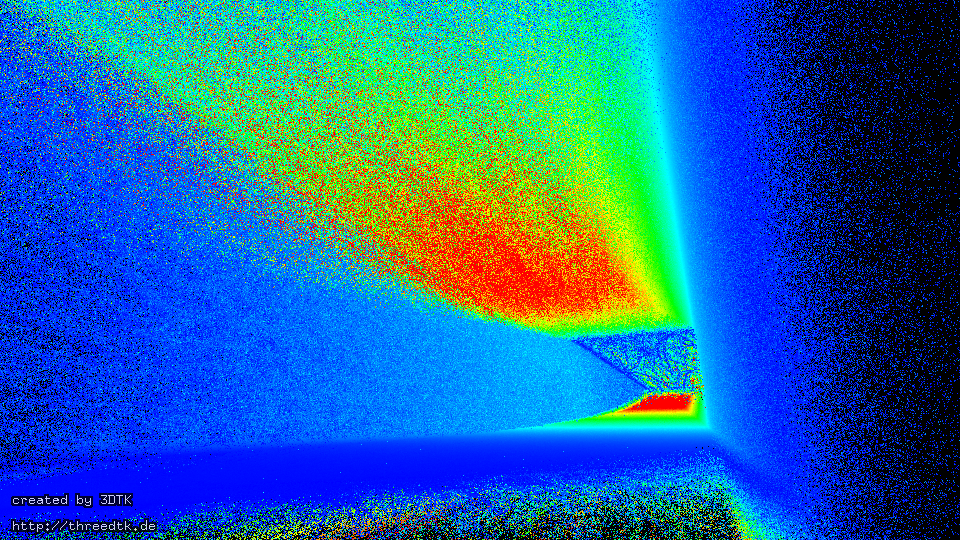
\includegraphics[width=\textwidth]{./images/uncorr_bottom_pose}\\
		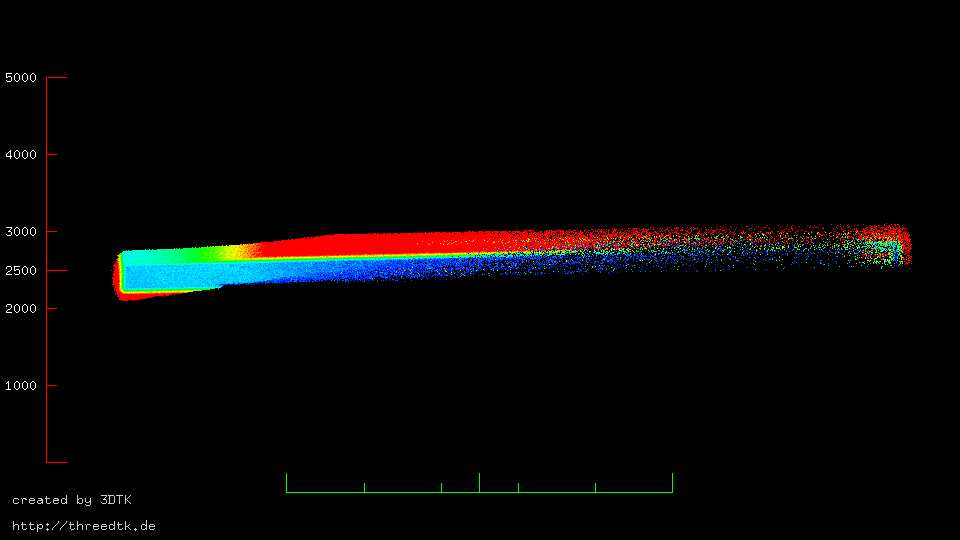
\includegraphics[width=\textwidth]{./images/uncorr_side_view}\\
  		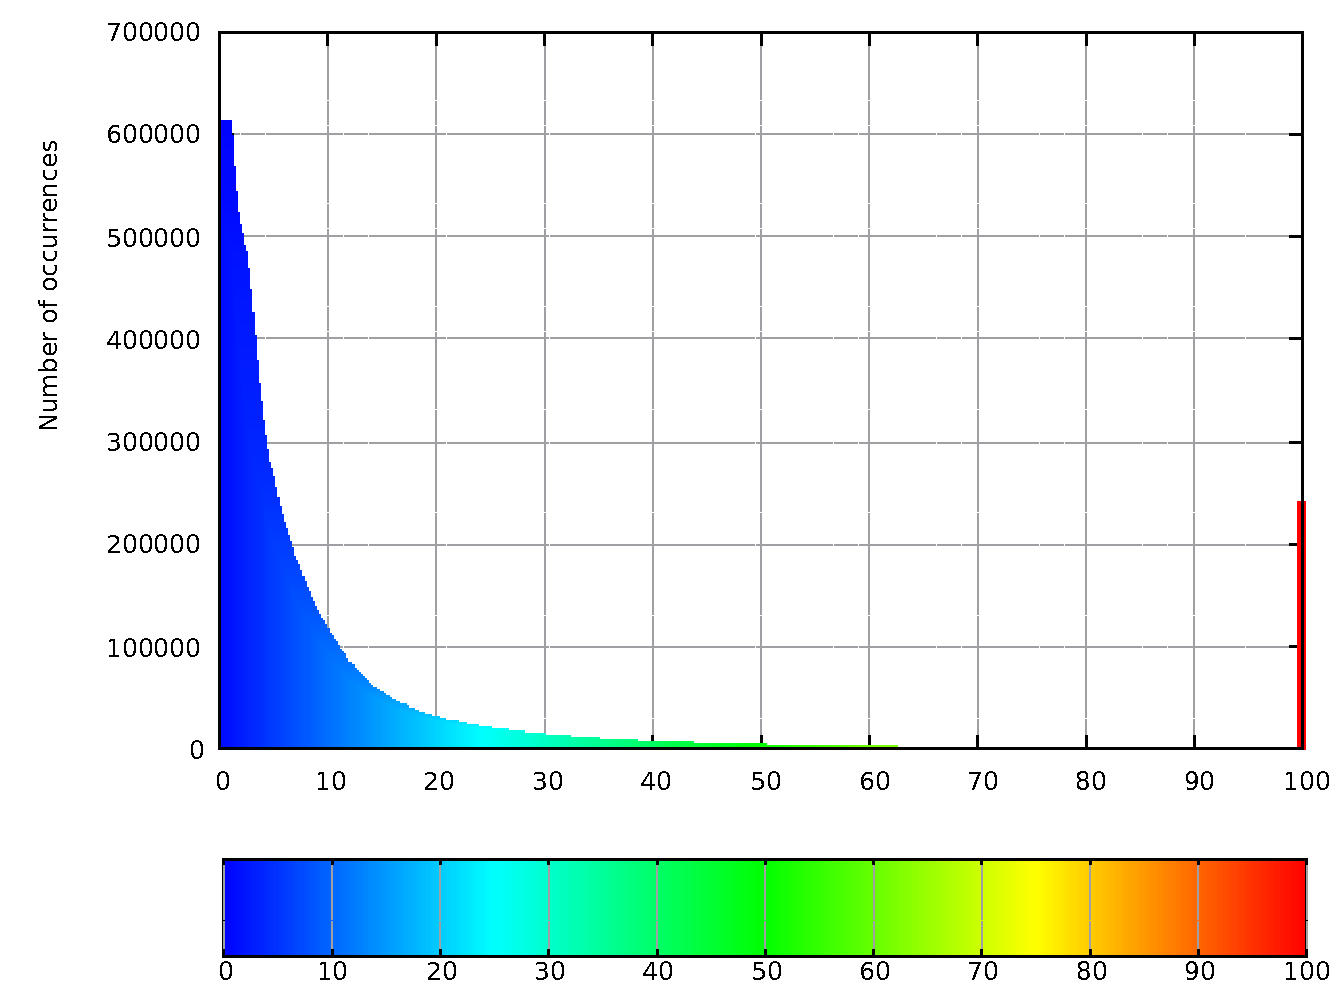
\includegraphics[width=\textwidth]{./images/uncorr_hist}
  	\end{minipage}\hfill
  	\begin{minipage}[c]{0.495\textwidth}
  		\centering
		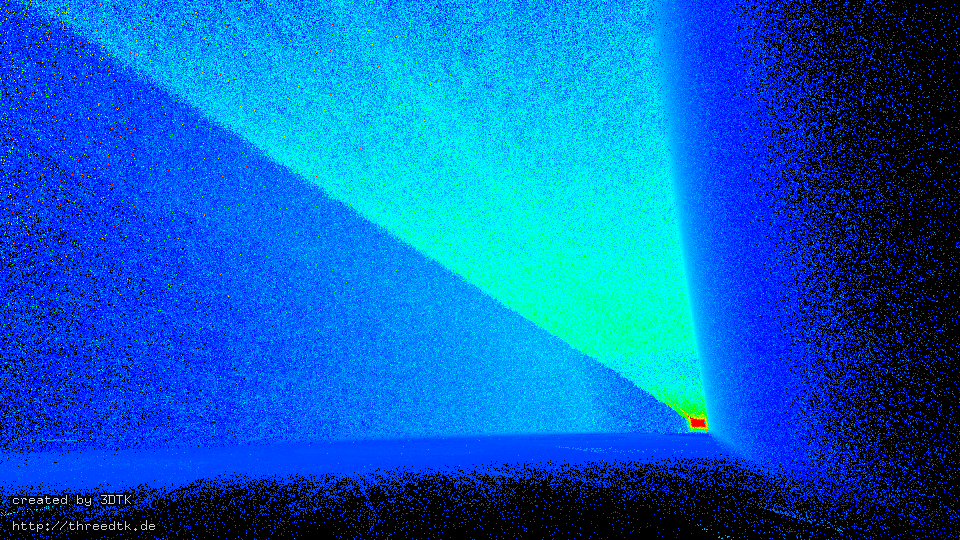
\includegraphics[width=\textwidth]{./images/corr_bottom_pose}\\
		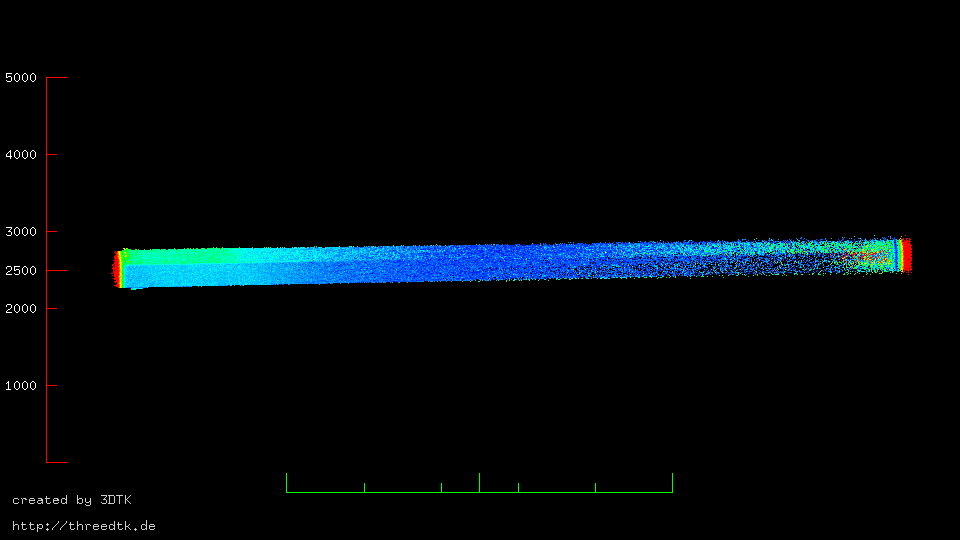
\includegraphics[width=\textwidth]{./images/corr_side_view}\\
  		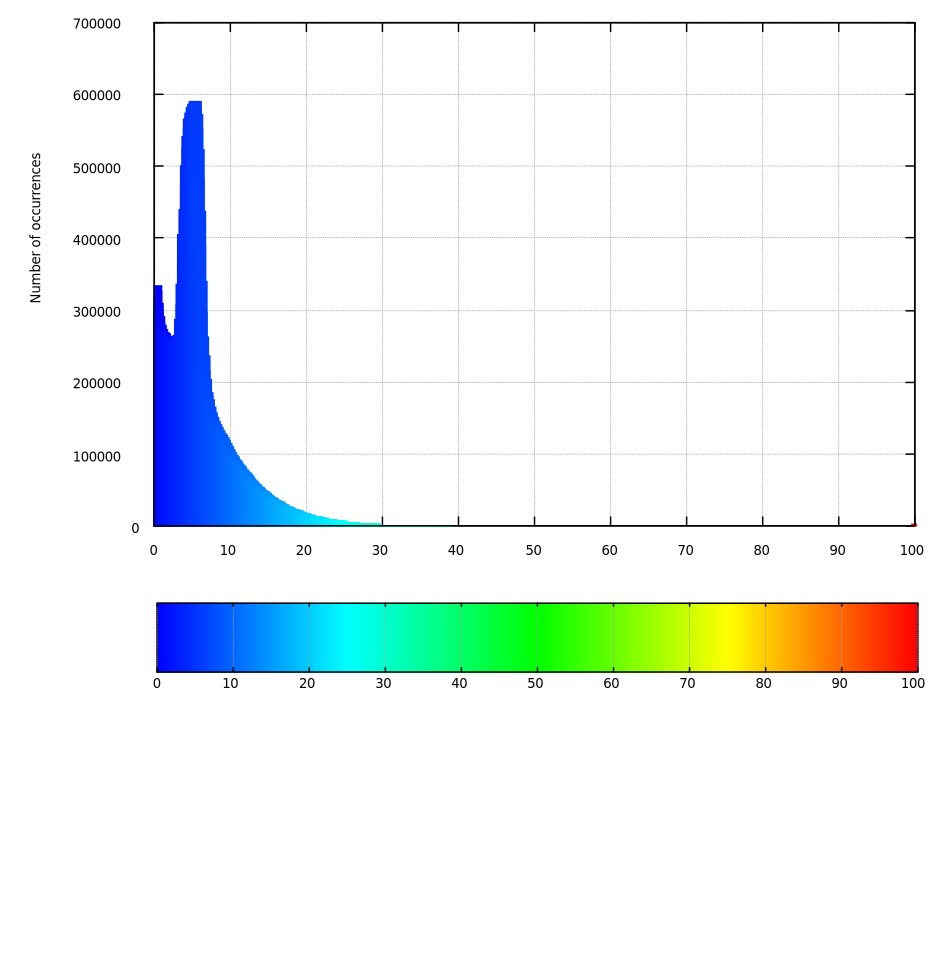
\includegraphics[width=\textwidth]{./images/corr_hist}
  	\end{minipage} 	
 	\caption{Evaluation of point distances before (left) and after (right) the plane-based registration on a simulated dataset. A maximal distance of \SI{2}{m} is set, such that all points that display a higher distance value are excluded from the analysis. Further, the histogram joins all values with a distance greater than \SI{1}{m} into the last bucket. The top two columns show a heat map of distances, while the bottom shows the corresponding histogram. The color mapping is equivalent in both. An animation of the matching process is given at \url{https://youtu.be/0ps5Pg4qo4E} .}
 	\label{fig:simulatedEvaluation}
\end{figure*} 

Before the registration, the corridor is only represented acceptably in the front part. 
The further into the corridor, i.e., the longer the robot accumulates errors, the more imprecise the data becomes. 
Finally, we see that a large portion of the data even exceeds either the \SI{1}{\meter} error, contributing to the large spike in the histogram or even the \SI{2}{\meter} error limit; thus, being cut from the representation. 
After registration, we see that, qualitatively, the ideal corridor was nearly restored from the noisy data. 
In particular a very large portion (95\%) have less than \SI{17}{\centi\meter} distances.
Further, the square and straight shape of the corridor is restored well, and especially the large spike at errors of greater than \SI{1}{m} is removed. 
Any such errors tend to occur at the back and the front of the corridor where the measured range is the largest hence has the largest contribution of the range error. 

\subsection{Floating Sphere Results}

Figure~\ref{fig:cylon-corrected} shows the results obtained before and after employing the plane based registration on the dataset acquired by the floating sphere.
We combine ten scans into one meta-scan, which is then globally registered.
This does not only speed up convergence due to the proportional effect on the error function but also decreases the risk of transforming the scan in a senseless way.
Transformations like these happen when incorrectly labeled points have a huge effect on the error gradient, which is especially the case when considering only a few points.

\begin{figure*}
	\centering
	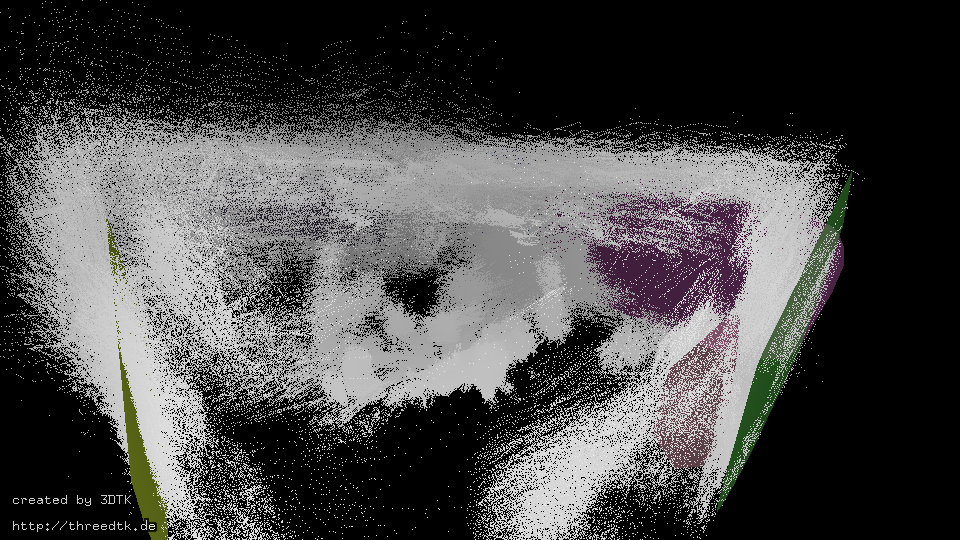
\includegraphics[width=0.495\textwidth]{./images/cylon_uncorr_corner}\hfill
	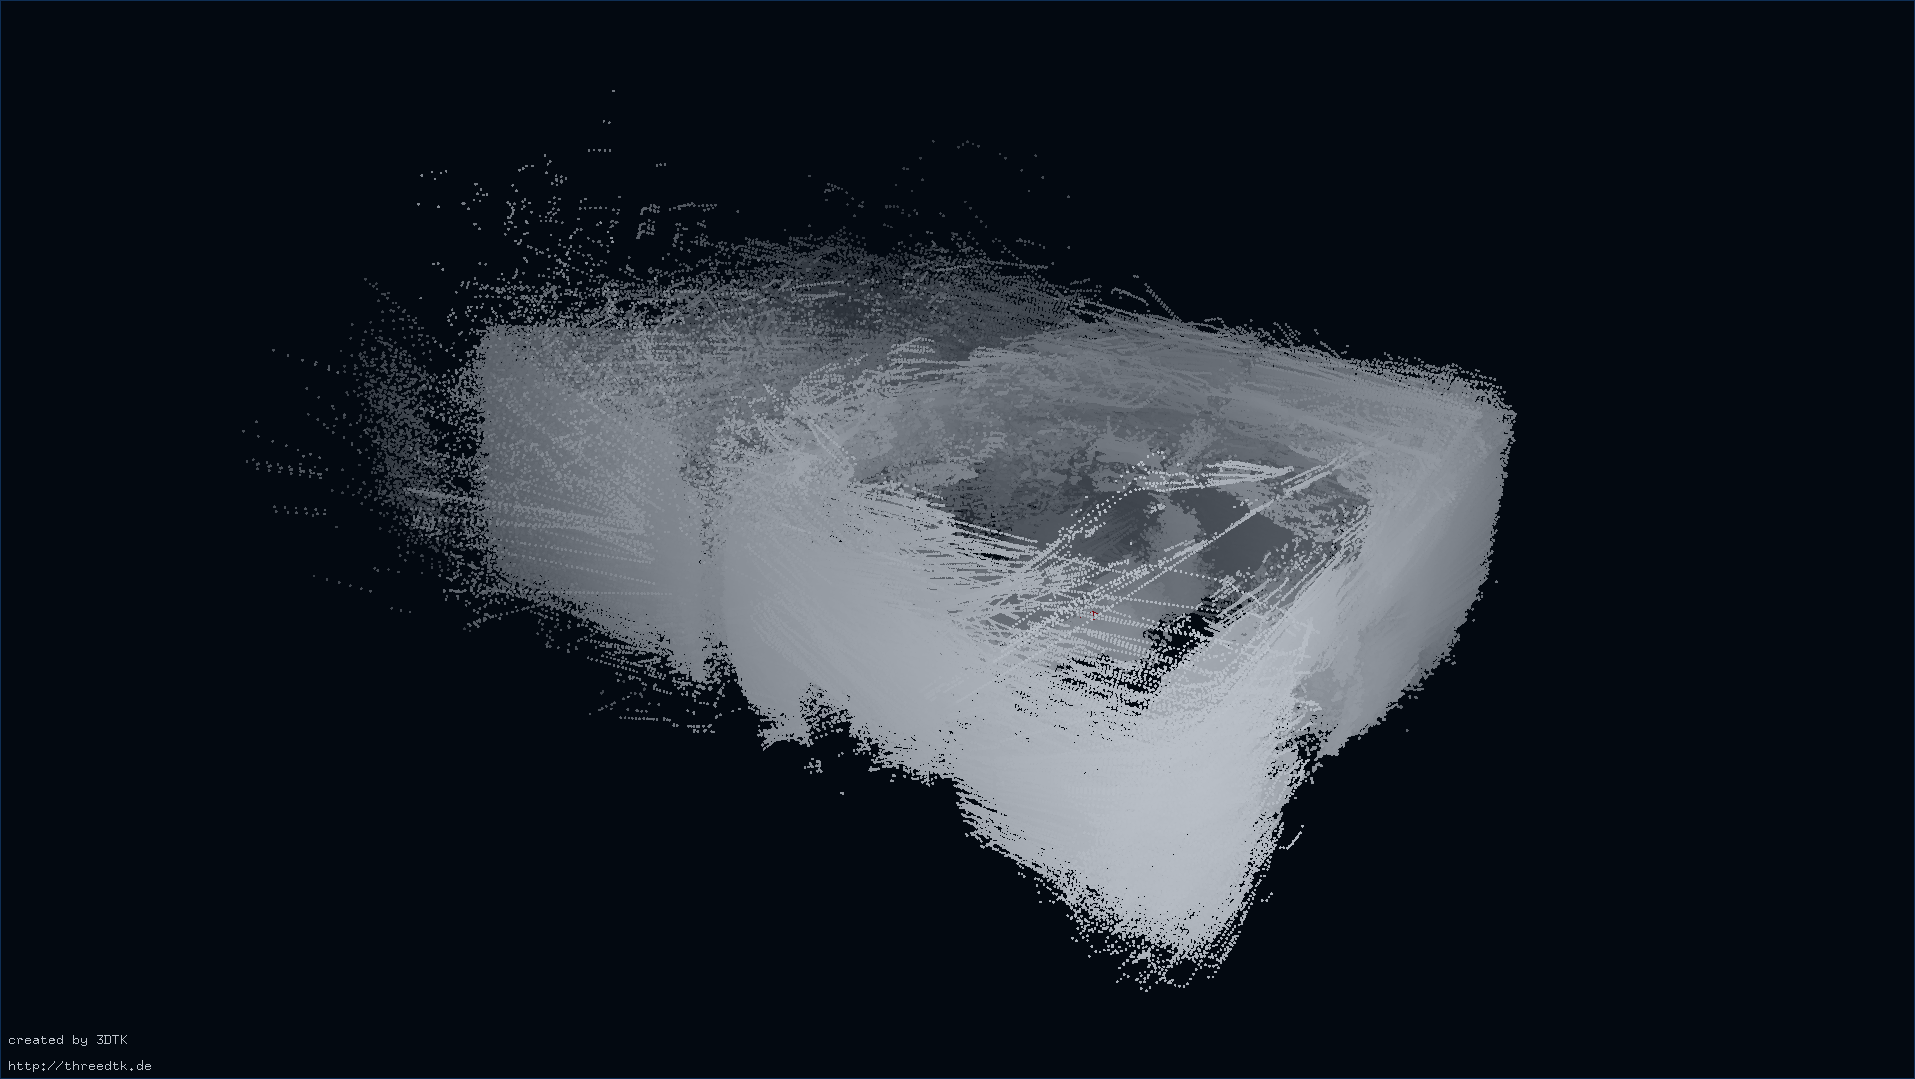
\includegraphics[width=0.495\textwidth]{./images/cylon_corr_corner}\\
	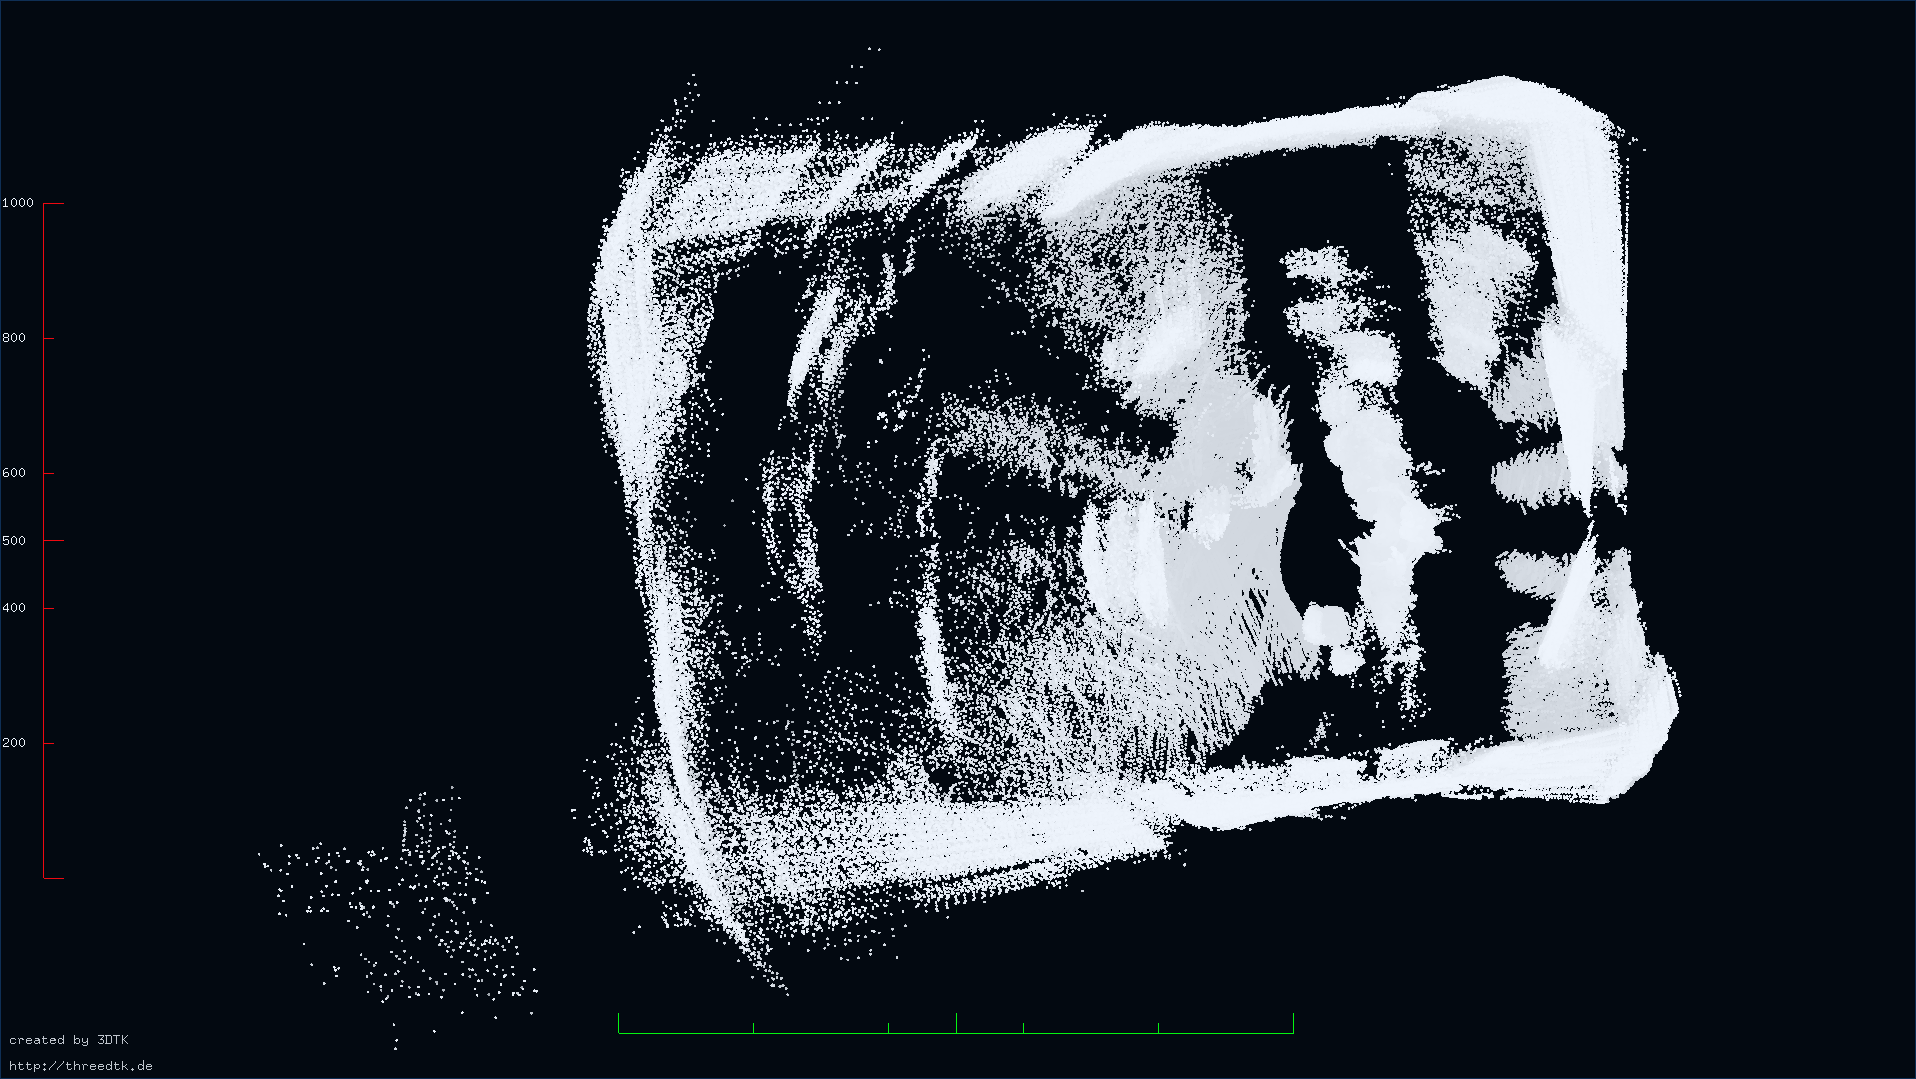
\includegraphics[width=0.495\textwidth]{./images/cylon_uncorr_top}\hfill
	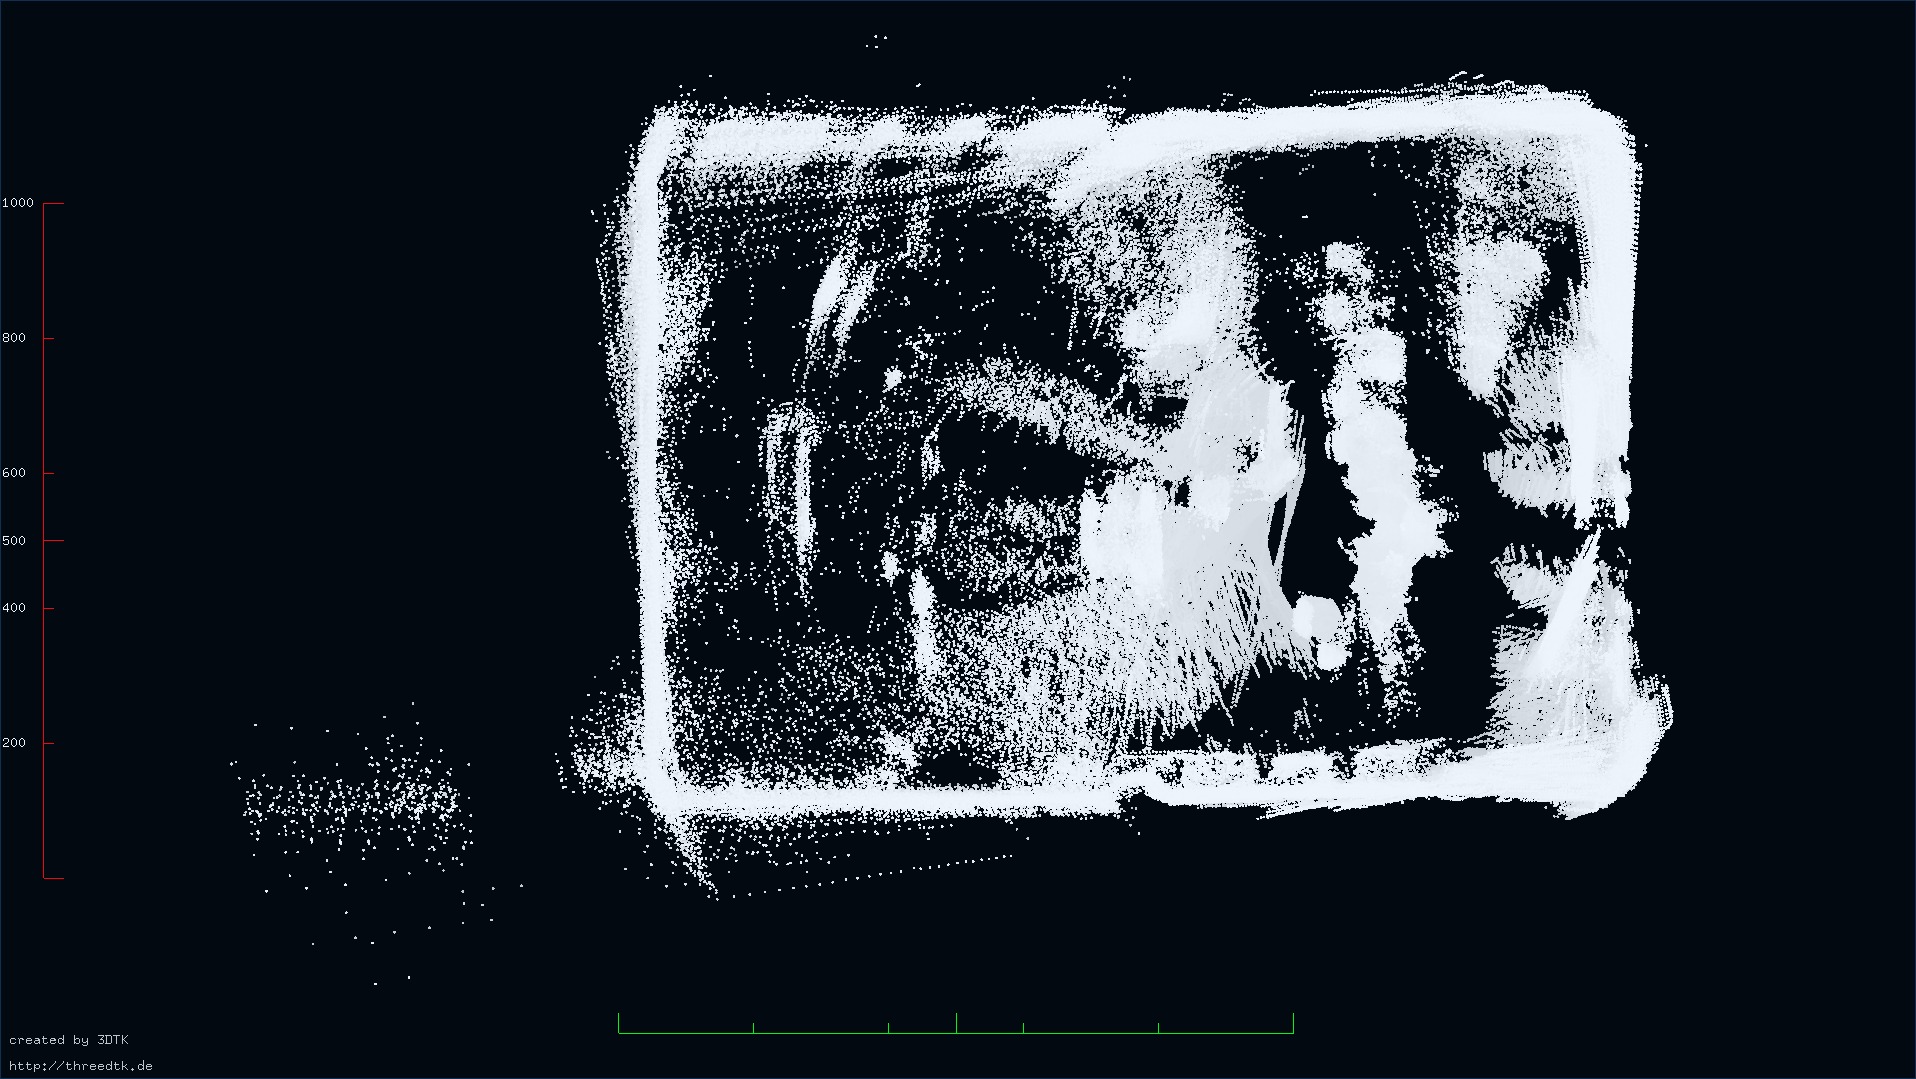
\includegraphics[width=0.495\textwidth]{./images/cylon_corr_top}
	\caption{The point cloud acquired by the floating sphere before (left) and after (right) applying the plane based registration. View from the interior that shows the used planes (top) and a birds-eye view (bottom). An animation of the registration process is given at \url{https://youtu.be/8XdIUN_9VpY} .}
	\label{fig:cylon-corrected}
\end{figure*}
After the registration, the walls of the room are significantly more prominent in the point cloud. 
In particular, the noise in the top left corner of the top view (cf. figure~\ref{fig:cylon-corrected}) has been visibly reduced.
Further, the deviation of points around the walls is notably smaller as the points are moved on the plane.

However, some imprecisions remain. 
In particular, at the initially very noisy top left corner of the top view, a few points cannot be matched to the plane. 
The scans that cause these imprecisions are problematic as they measure a number of plane-like structures in the interior of the room. 
When relabeling those scans, the interior points are associated with a plane, and hence the corresponding distance is minimized. 


% This section is commented out
\iffalse
\subsection{RADLER Results}

\subsection{Experimental Results REMOVE THIS SECTION}

For the experimentally acquired datasets a similar procedure is followed. 
The main difference being, that the scan was pre-registered using a point-to-point based method as described in section~\ref{sec:experimentalSetup}. 
Here also the point distances to the ground truth (in this case the terrestrially acquired 3D laser scan) is evaluated before and after the plane-based registration process. 

\begin{figure}
	\centering
	\begin{minipage}[c]{0.25\textwidth}
		\centering	
		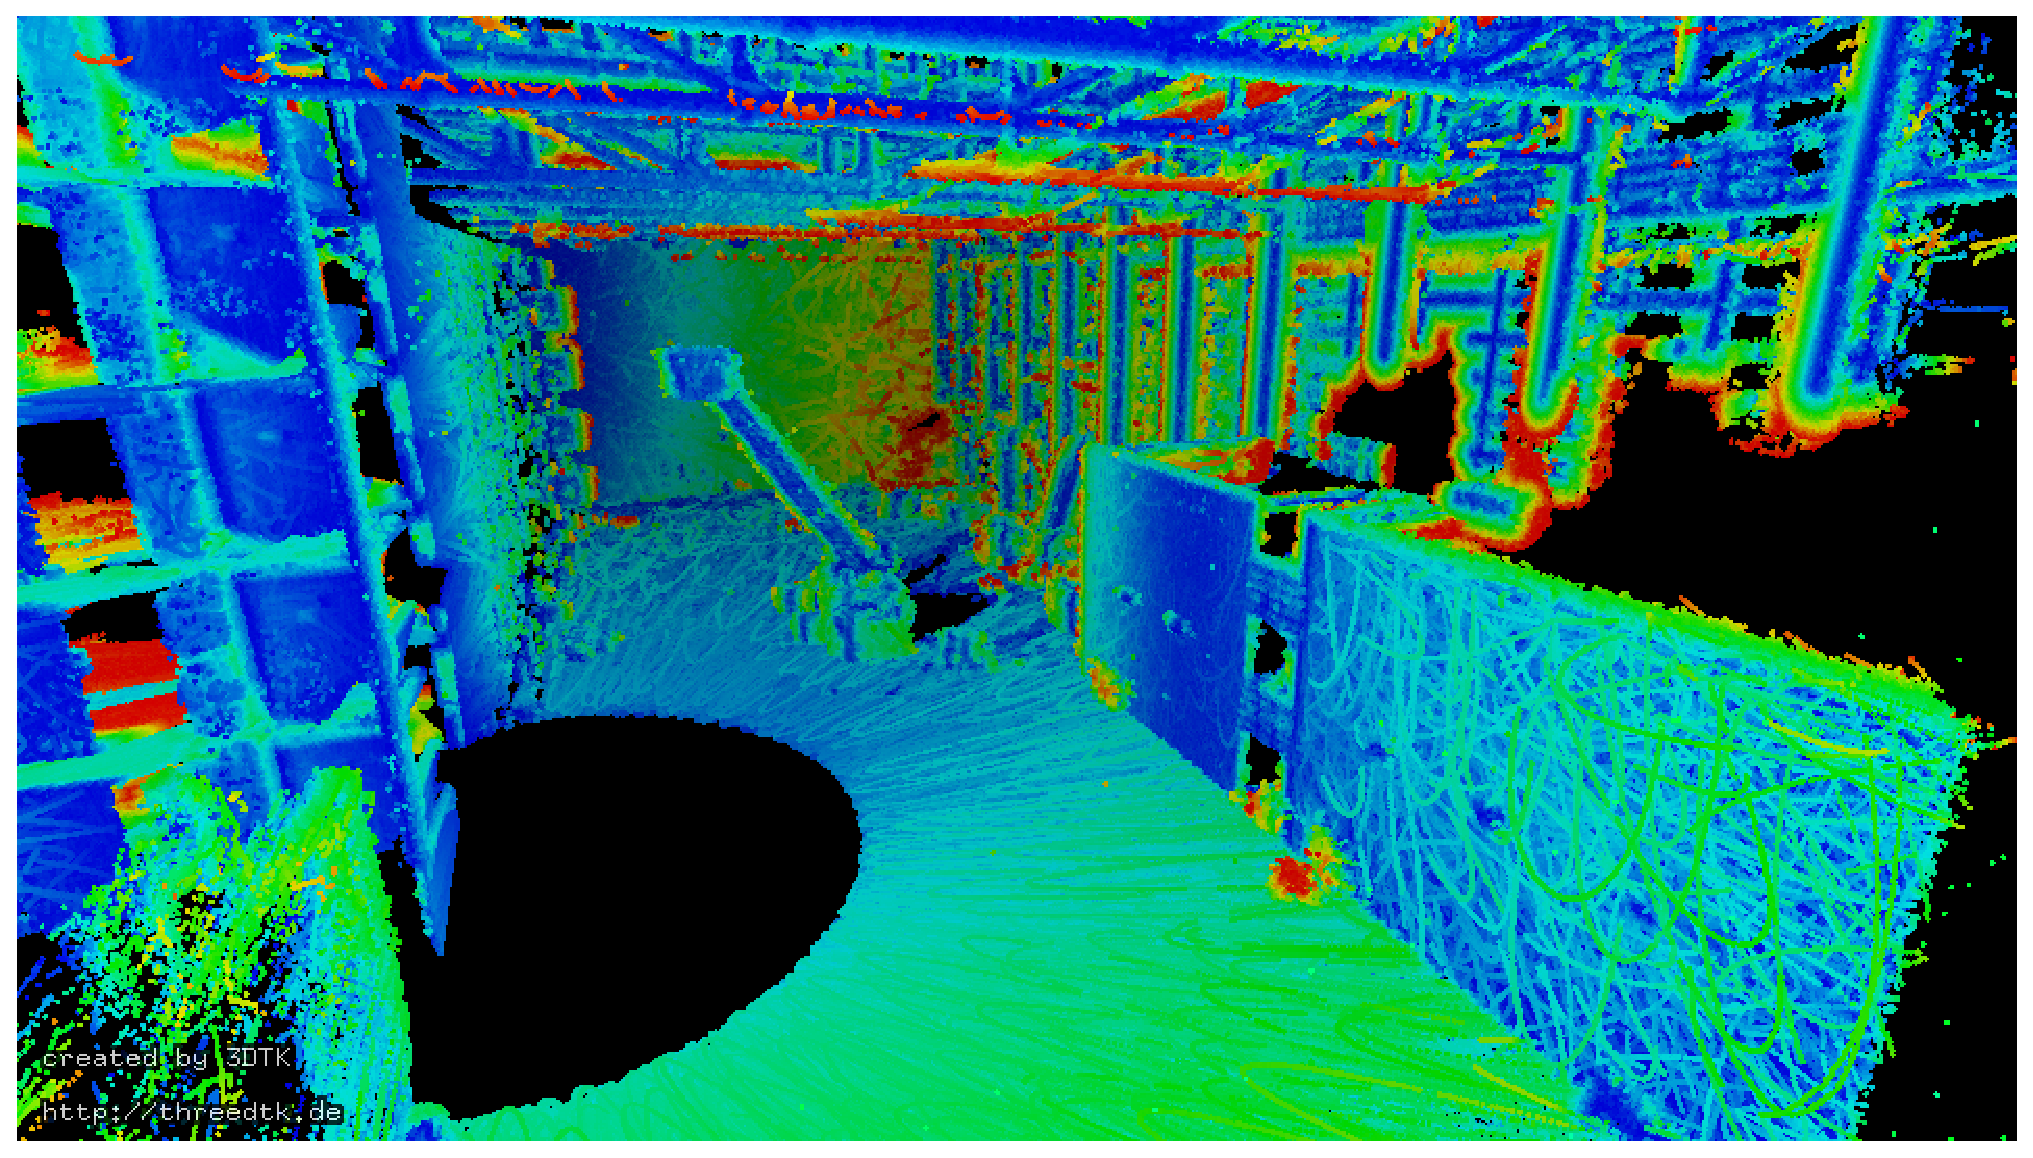
\includegraphics[width = \textwidth]{./images/distances_fire}\\
		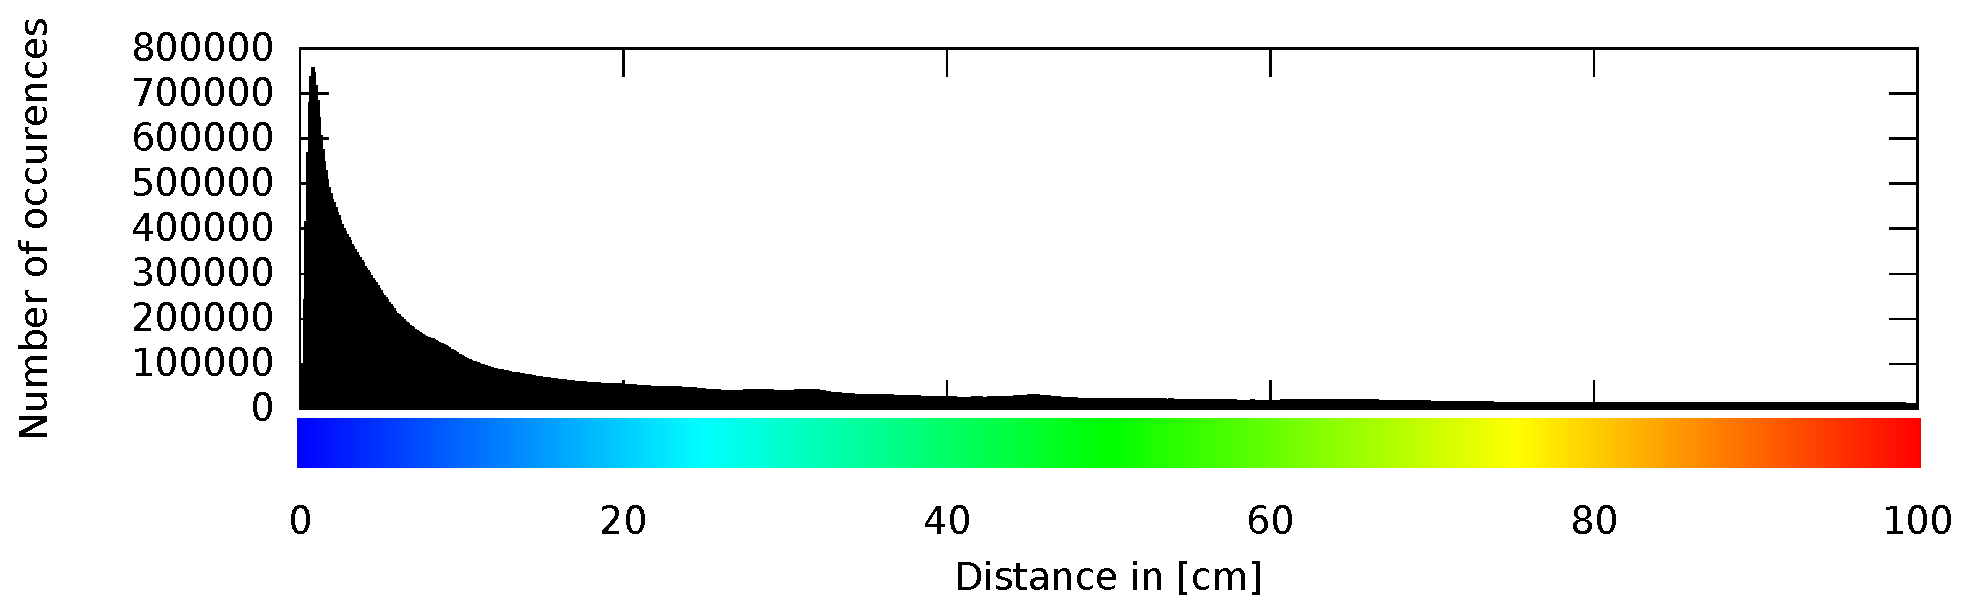
\includegraphics[width = \textwidth]{./images/histogram_fire}
  	\end{minipage}\hfill
  	\begin{minipage}[c]{0.25\textwidth}
  	\end{minipage} 	

	\todo[inline]{Evaluate Plane matching on firefighter school data; histogram after etc}
	\caption{Evaluation of point distances before (left) and after (right) the plane based registration on a experimentally acquired dataset. A maximal distance of \SI{5}{m} is set, such that all points that display a higher distance value are excluded. The left column shows a heat map of distances while the right shows the corresponding histogram. The color mapping is equivalent in both. An animation of the matching process can be seen \href{todo}{here}}
	\label{fig:experimentalEvaluation}
\end{figure}
\fi
